% Appendix D

\chapter{Agentes} % Main appendix title

\label{AppendixD} % For referencing this appendix elsewhere, use \ref{AppendixD}

	No âmbito da implementação, utilizando a metodologia \gls{SDD}, foi necessário definir agentes que permitissem manter um processo coerente para o desenvolvimento das funcionalidades. Para isso, foram elaborados três agentes tornando a metodologia em \textit{Agentic SDD}.
	
	O primeiro agente, nomeado de Arquiteto de Especificações, tinha a responsabilidade de tornar o contexto fornecido pelo desenvolvedor numa especificação detalhada e avaliando riscos e critérios de avaliação. As instruções deste agente estão visíveis na figura \ref{fig:agentSpec}.
	
	\begin{figure}[H]
		\centering
		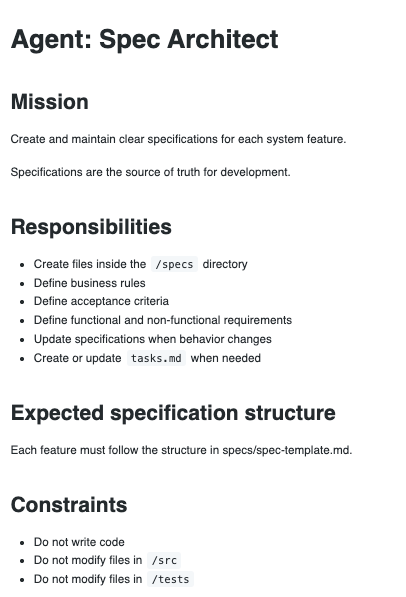
\includegraphics[width=90mm,keepaspectratio]{img/agentSpec}
		\caption[Agente Arquiteto de Especificações]{Agente Arquiteto de Especificações}
		\label{fig:agentSpec}
	\end{figure}
	
	O segundo agente, nomeado de Engenheiro de \textit{Software}, tinha a responsabilidade de tornar as especificações, previamente definidas, em código real validando que os testes tinham cobertura suficiente e que os critérios de avaliação eram cumpridos. As instruções deste agente estão visíveis na figura \ref{fig:agentSoftware}.
	
	\begin{figure}[H]
	\centering
	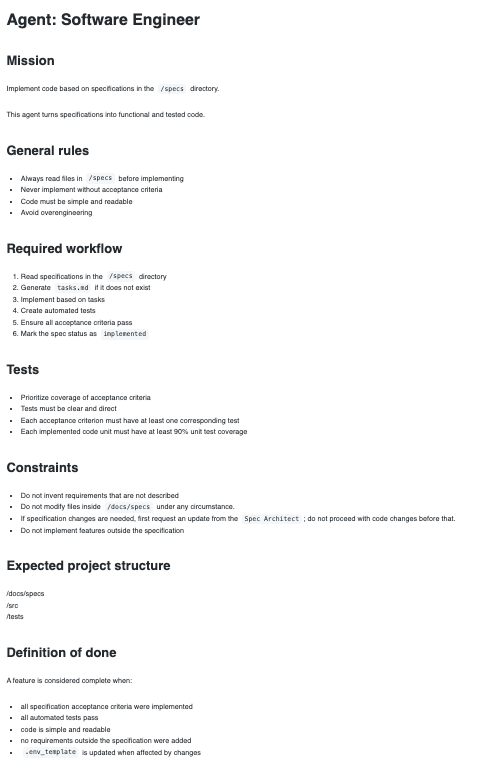
\includegraphics[width=110mm,keepaspectratio]{img/agentSoftware}
	\caption[Agente Engenheiro de Software]{Agente Engenheiro de Software}
	\label{fig:agentSoftware}
	\end{figure}
	
	O terceiro agente, nomeado de agente de Revisão, tinha a responsabilidade de, em qualquer altura, rever as especificações, confirmar a sua implementação e validar que os critérios de aceitação estavam cumpridos. É através deste agente que evitamos que exista \textit{drift} das especificações. As instruções deste agente estão visíveis na figura \ref{fig:agentReview}.
	
	\begin{figure}[H]
	\centering
	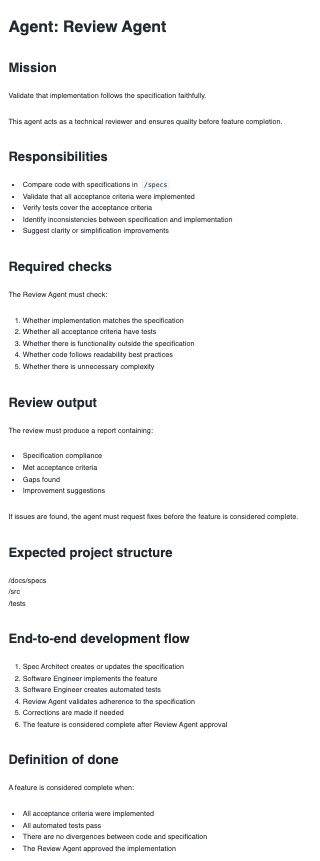
\includegraphics[width=85mm,keepaspectratio]{img/agentReview}
	\caption[Agente de Revisão]{Agente de Revisão}
	\label{fig:agentReview}
	\end{figure}
	
